\documentclass{aa}
%\documentclass[referee]{aa}
%\usepackage[top=0.75in, bottom=0.5in, left=1in, right=1in]{geometry}
%\usepackage[titletoc]{appendix}
\usepackage[varg]{txfonts}
\usepackage{amsmath}
\usepackage{amssymb}
\usepackage{mathrsfs}
%\usepackage{natbib}
\usepackage{aas_macros}
%\usepackage{fancyvrb}
\usepackage{gensymb}
\usepackage{appendix}
\usepackage{multirow}
\usepackage[font=small,labelfont=bf]{caption}

%\newcommand{\refrevision}[1]{\textbf{#1}}
\newcommand{\refrevision}[1]{#1}
%\newcommand{\refrevisiona}[1]{\textbf{#1}}
\newcommand{\refrevisiona}[1]{#1}

% Graphics type
\usepackage{graphicx}

\newcommand\prox{Proxima~Centauri}
\newcommand\bstar{Barnard's~Star}
\newcommand\ross{Ross~154}
\newcommand\rdwarf{M-dwarf}
\newcommand\ldwarf{L-dwarf}
\newcommand{\bvec}[1]{\mbox{\boldmath ${#1}$}}
\newcommand{\rmsub}[2]{#1_{\rm #2}}
\newcommand{\dex}[1]{\hbox{$\times\hbox{10}^{#1}$}}
\newcommand{\rsun}{\,\mbox{$\rm R_{\odot}$}}
\newcommand{\rjup}{\,\mbox{$\rm R_J$}}
\newcommand{\msun}{\,\mbox{$\rm M_{\odot}$}}
\newcommand{\mearth}{\,\mbox{$\rm M_{\oplus}$}}
\newcommand{\rearth}{\,\mbox{$\rm R_{\oplus}$}}
\newcommand{\mjup}{\,\mbox{$\rm M_J$}}
\newcommand{\lsun}{\,\mbox{$\rm L_{\odot}$}}
%\newcommand{\ion}[2]{#1{\sc{\romannumeral #2}}}
\newcommand{\chem}[2]{\hbox{$^{#2}$}#1}
\newcommand{\kms}{\hbox{kms$^{-1}$}}
\newcommand{\ms}{\hbox{ms$^{-1}$}}
\newcommand{\cms}{\hbox{cms$^{-1}$}}
\newcommand{\vsini}{\hbox{$v$\,sin\,$i$}}
\newcommand{\vs}{\hbox{$v$\,sin\,$i$}}
\newcommand{\rsini}{\hbox{$R$\,sin\,$i$}}
\newcommand{\vrad}{\hbox{$v_{rad}$}}
\newcommand{\degs}{$\degr$}
\newcommand{\chisq}{$\chi^{2}$} 
\newcommand{\radsec}{rad s$^{-1}$}
\newcommand{\radday}{\hbox{rad.day$^{-1}$}}
\newcommand{\invday}{\hbox{day$^{-1}$}}
\newcommand{\ha}{H$\alpha$}
\newcommand{\hb}{H$_{\beta}$}
\newcommand{\hg}{H$_{\gamma}$}
\newcommand{\rhk}{Log(R'HK)}

\newcommand{\asas}{{\sc asas}}
\newcommand{\uves}{{\sc uves}}
\newcommand{\hst}{{\sc hst}}
\newcommand{\ktwo}{{\sc k2}}
\newcommand{\MEarth}{{\sc MEarth}}
\newcommand{\rem}{{\sc rem}}

\newcommand{\scipy}{{\sc scipy}}
\newcommand{\astroml}{{\sc astroml}}
\newcommand{\gatspy}{{\sc gatspy}}
\newcommand{\matplot}{{\sc matplotlib}}

% So we can change our minds what to call them

\newcommand\Notnow[1]{}

% Stuff different between paper and thesis, this is for paper
% ===========================================================

\newcommand\IfPaper[1]{#1}
\newcommand\IfThesis[1]{}
\newcommand\PaperThesis[2]{#1}
\newcommand\paperorthesis{paper}
\newcommand\FirstP{We}
\newcommand\Firstp{we}
\newcommand\Firstobj{us}
\newcommand\Firstposs{our}
\newcommand\FirstPoss{Our}

\begin{document}

\title{Calculations of periodicity from various light curve data of {\ross}}

\author{John M. Collins\inst{\ref{uherts}}\and Hugh R.A. Jones\inst{\ref{uherts}}
\and Ben Burningham\inst{\ref{uherts}}\and John R. Barnes\inst{\ref{openu}}}

\institute{University of Hertfordshire, College Lane, Hatfield, Herts, AL10 9AB, UK\label{uherts} \and 
Department of Physical Sciences, The Open University, Walton Hall, Milton Keynes, MK7 6AA, UK\label{openu}}

\date{\today}

\abstract{{\FirstP} investigate retrieval of periodic data, in particular the
stellar rotation signal for {\ross}. {\FirstP} make use of light curve data
taken from a variety of sources including K2, ASAS and also derived by the
authors from observations via the REM automatic telescope in La silla, Chile.}

\keywords{Stars: late-type --- Line: rotation period --- Methods: miscellaneous}

\maketitle

\protect\label{firstpage}

\section{Introduction}
\protect\label{section:intro}

{\ross} is 2.976 pc distant, of spectral type M3.5. It has a reasonably high
proper motion of $-637.02$ mas/yr in Right Ascension and  {–}191.64 mas/yr
in Declination and a radial velocity of {–}10.7 km/s \citep{vanleeuwen07}. It is
notable for its strong activity, for example in \citet{wargelin08} and it is
well-understood that activity is associated with a fast rotation period,
especially in \rdwarf s, for example in \citet{mohanty03}.

As part of a project to analyse automatically-collected data from the {\rem}
telescope in La Silla, Chile, further described below in Section
\ref{section:rem}, which covers 3 \rdwarf s including \ross, existing data for
those stars were studied. It appeared that there were some omissions and
discrepancies between the various tabulations of parameters for \ross, which
this paper seeks to address.

\subsection{Data relevant to \ross}

For the purposes of discussion in this paper, the following parameters for
{\ross} are of particular interest.

\begin{enumerate}
  \item The radius.
  \item The rotational velocity \vsini.
  \item The rotation period.
\end{enumerate}

These are all inter-related, in that the rotational velocity (without the factor of
the sine of the inclination) is related to the others by $v = \frac{2 \pi
r}{t}$, where $v$ is the ``true'' rotational velocity as opposed to the
projected rotational velocity, \vsini, $r$ is the radius and $t$ is the rotation
period.

\subsubsection{Values for radius}

The radius of a star is calculated by determining the bolometric luminosity and
the temperature and applying the black-body radiation formula $L = 4 \pi R^2
\sigma T^4$, where L is the luminosity, which can be derived from the absolute
magnitude, T is the temperature in {\degree}K and $\sigma$ is the
Stephan-Boltzmann constant.

A radius was previously given in \citet{pettersen80} of $1.5 \pm 0.2 \times 10^8$ m, which equates to $0.22 \pm
0.03$\rsun. A larger radius of $0.24 \pm 0.06$ {\rsun} is given in \citet{johnson83}
\footnote{\citet{johnson83} do not explicitly state the
uncertainty, but gives a limit of 25\% for results not studied in more detail
from which this uncertainty was calculated.}.

A much more recent study, \citet{pineda21} has proposed a radius of $0.200 \pm
0.008$ \rsun. The discrepancies between these values are accounted for by
refinements to the measurements of bolometric luminosity and the effective
temperature. In the latter paper these.are given as $1.537 \pm 0.018
\times 10^31$ erg/s\footnote{This is equivalent to $0.00402 \pm 0.00005$\lsun.}
and $3248^{+68}_{-66}$K.

There does appear to be considerable variation in the values for bolometric
luminosity and/or magnitude between papers and also in the effective
temperature, which accounts for the considerable variation in values.

\subsubsection{Rotational velocity \vsini}

As with the radius, there is some variation in the rotational velocity \vsini.

A value of $3.5 \pm 0.5$ km/s is given in \citet{johnskrull96} and quoted in
\citet{wargelin08} who state that the fast rotation period is indicative of an
age of less than 1 Gyr. The period of rotation is not stated there.
\citet{reiners18} report a value for {\vsini} of $3.0 \pm 1.5$ km/s, whilst
\citet{hojjatpanah19} report a figure of $5.20 \pm 0.91$.

These figures are all obtained from spectral line broadening. It is possible
that the star's known considerable activity might contribute to this yielding an
overestimate.

\subsubsection{Rotation period}

The value of the rotational velocity sets an upper limit on the rotation period.
If the inclination of the star is less than 90{\degree}, then the projected
rotational velocity {\vsini} will be lower than the actual rotational velocity
by the factor of the sine of the inclination.

Using the formula $t = \frac{2 \pi r}{v}$ and assuming a radius $r$ of
0.200\rsun, an upper limit on the rotation period is obtained of 2.891 days if
the value of {\vsini} of 3.5 km/s is assumed, 3.373 days if 3.0 km/s is assumed
and 1.946 days if 5.2 km/s is assumed.

The literature reports varying calculations of the rotation period.
Previously, in \citet{jarrett76}, an activity cycle of about 2 days was reported, but
possibly this might have been confused with the rotation period. 
A period of 2.869 days is given in \citet{kiraga07}, one of 2.857
or 2.843 days (taken from {\ktwo} or {\MEarth} respectively) in \citet{newton18},
$4.7 \pm 2.3$ days in \citet{reiners18}\footnote{This cannot be credible as the
figure for {\vsini} also given by this paper of $3.0 \pm 1.5$ km/s sets an
upper limit of the rotation period of 3.373 days.} and $2.87 \pm 0.01$ days in
\citet{diezalonso19}, based on {\asas} data.

\subsection{Aims of this study}

In view of the plethora of statistics for \ross, it would be useful to confirm
or refine the figure for the rotation period as no planets have been reported for {\ross}
and a low inclination angle might be one of the
reasons for the difficulty in detection which would be indicated if the maximum
rotation period indicated by (\vsini) was significantly more than the detected
rotation period.

As the authors were considering the visible light observations of the {\rem}
telescope, a study of the rotation period was undertaken using the various data
sources referred to in the above papers and the results presented herein.

\section{Periodograms from various sources of data}
\protect\label{section:variousrot}

Using data from the various papers referred to above, attempts were made to
recover periodic data from the various sources referred to and also from data
associated with the goal of this project, the {\rem} telescope.

\subsection{Study of data from \ktwo}
\protect\label{section:k2data}

Data from {\ktwo} was only available for a single 80-day period starting on 15
October 2005. This showed an interval at the start strongly affected by frequent
flaring events, however there was a quiescent period during which a regular
cyclic pattern could be observed, for example as seem in
Fig. \ref{fig:k2all} with the latter part in Fig. \ref{fig:k2lcurve}.
This last part shows a clear periodic cycle
which can be used to generate a very clear periodogram as shown in Fig.
\ref{fig:k2pgram}, with a very prominent peak at 2.87 days. A light curve folded
on this period is shown in Fig. \ref{fig:k2pfold}. The display starts at 2 days,
as the window function of the time series, as shown in Fig. \ref{fig:k2winfunc},
shows significant peaks in the periods below this.

\begin{figure}[!htbp]
\begin{center}
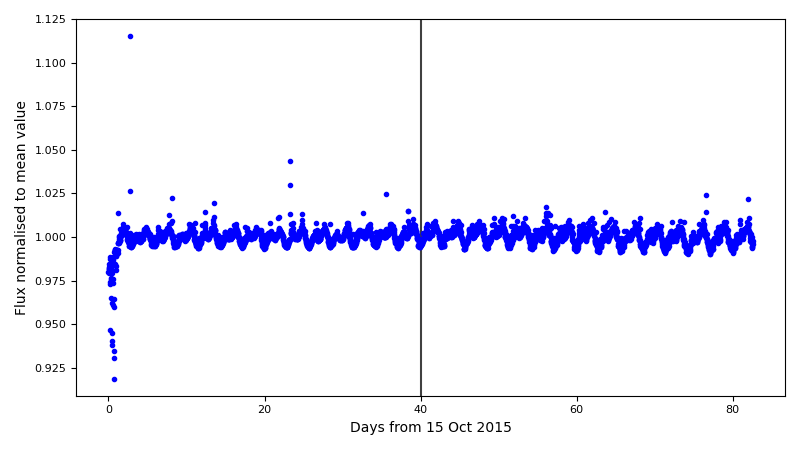
\includegraphics[scale=0.40]{k2/images/k2all.png} \\
\vspace{-.5cm}
\end{center}   
\caption{Scatter plot of observed flux for {\ross} taken from the archive of
{\ktwo} data on MAST for 10 October 2015 onward. The error bar is too small to
display. The first part appears to be affected by some diminution in activity or
error and in subsequent analysis, the portion to the right of the vertical line
set at 40 days is taken.}\protect\label{fig:k2all}
\end{figure}

\begin{figure}[!htbp]
\begin{center}
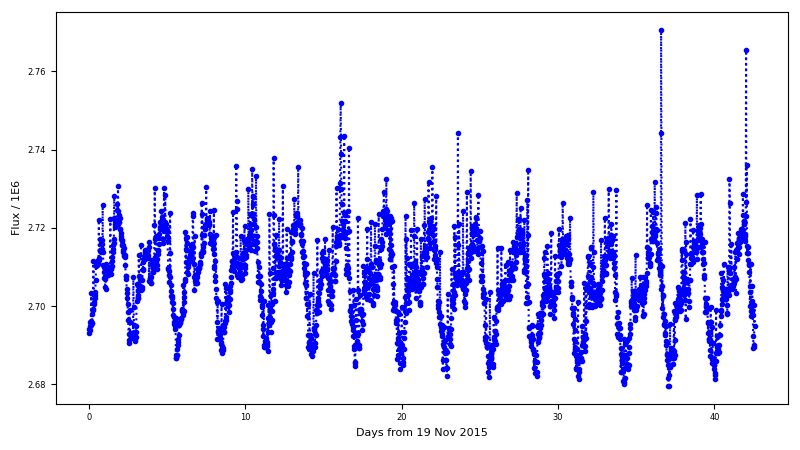
\includegraphics[scale=0.40]{k2/images/k2lcurve.png} \\
\vspace{-.5cm}
\end{center}   
\caption{Scatter plot of observed flux for {\ross} taken from the archive of
{\ktwo} data on MAST for 10 October 2015 onward, omitting the first 40 days,
which appear, especially at the beginning, to be affected by a significant
reduction in activity, and also outlying data of greater than 2 standard deviations.
Again, the error bar is too small to display.}\protect\label{fig:k2lcurve}
\end{figure}

\begin{figure}[!htbp]
\begin{center}
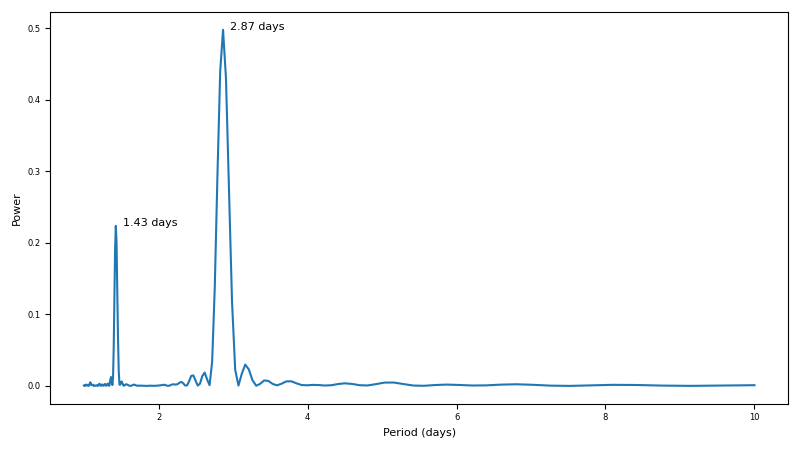
\includegraphics[scale=0.40]{k2/images/k2_pg.png} \\
\vspace{-.5cm}
\end{center}   
\caption{Periodogram taken from the data displayed in Fig.
\ref{fig:k2lcurve} but not omitting outlying data
greater than 2 standard deviations, which made
little difference to the result. There were additional peaks of less than a day
to be observed, however these have been omitted as there were aliases of the
2.87 day period, observed from the emulations described below, which conflicted
with these.} \protect\label{fig:k2pgram}
\end{figure}

\begin{figure}[!htbp]
\begin{center}
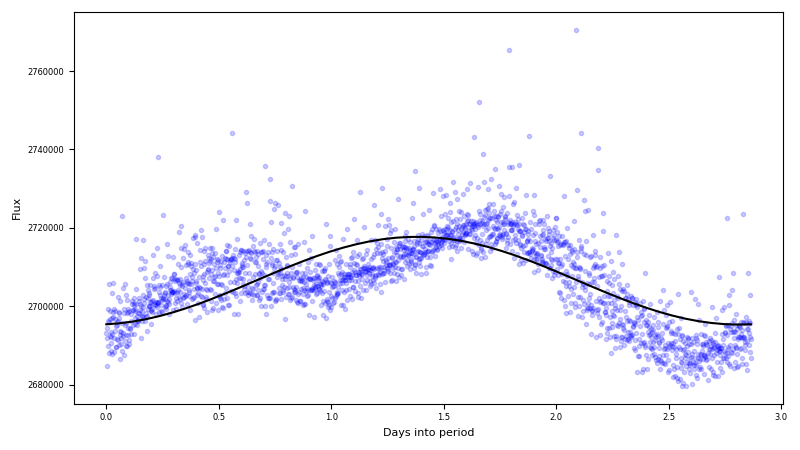
\includegraphics[scale=0.40]{k2/images/k2_pfold.png} \\
\vspace{-.5cm}
\end{center}   
\caption{Light curve taken from the data displayed in Fig.
\ref{fig:k2lcurve} folded on the main peak of 2.87 days displayed in Fig.
\ref{fig:k2pgram}. Points exceeding 2 standard deviations from the mean are
omitted for clarity of display.} \protect\label{fig:k2pfold}
\end{figure}

\begin{figure}[!htbp]
\begin{center}
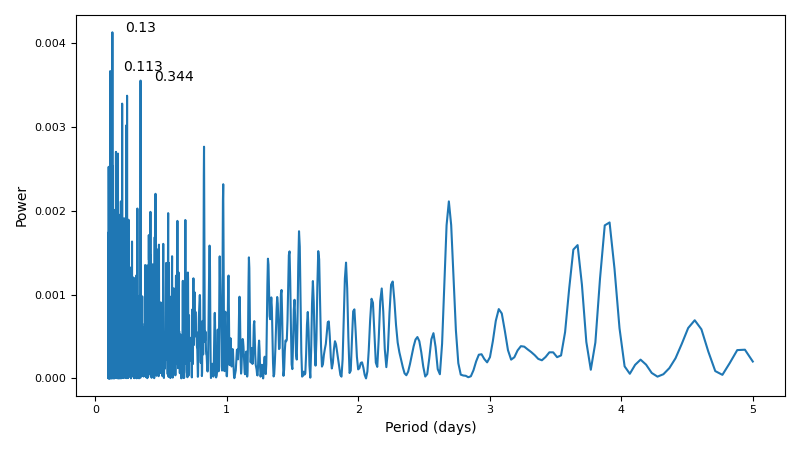
\includegraphics[scale=0.40]{k2/images/k2winfunc.png} \\
\vspace{-.5cm}
\end{center}   
\caption{Window function of the time series for the {\ktwo} data showing numerous
peaks in the period space below 2 days.} \protect\label{fig:k2winfunc}
\end{figure}

On the hypothesis that there were patterns of bright or dark spots on the face
of {\ross} which were relatively static over a period of a few days, like the
Sun, a very simple model, using the same time parameters as with Fig.
\ref{fig:k2lcurve} and Fig. \ref{fig:k2pgram}, was run yielding the result in
Fig. \ref{fig:k2emulated}. Results, as will be apparent, were virtually
identical to those from the {\ktwo} data for \ross, even though the simulated
noise on the values for the flux was ramped up to worse than 50 to 1, far worse for
that for the {\ktwo} data, the mean SNR of which was better than 40,000 to 1.
Whatever pattern on light or dark data, other than artificially cyclical data,
yielded the same periodogram.

Both the ``real'' periodogram and the emulated one showed strong peaks of less
than 1 day which have to be aliases of the 2.87 period and prevent any
meaningful analysis of periods less than 1 day which might be suggested by the
format of the cycles observed in Fig. \ref{fig:k2lcurve}.

\begin{figure}[!htbp]
\begin{center}
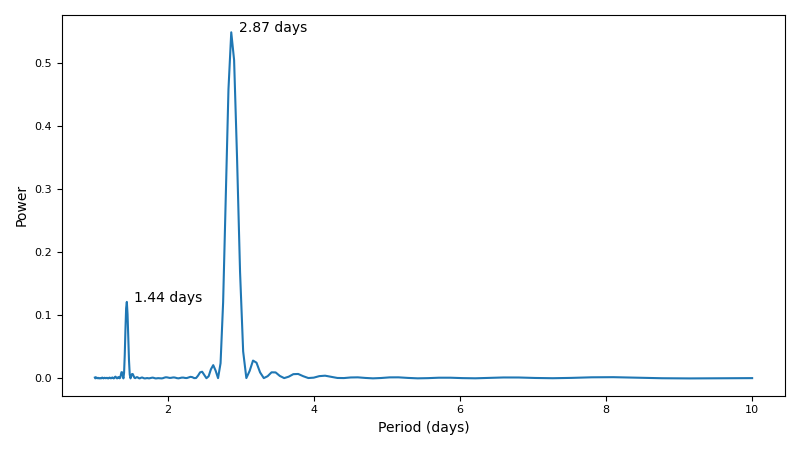
\includegraphics[scale=0.40]{k2/images/k2emulated.png} \\
\vspace{-.5cm}
\end{center}   
\caption{Periodogram generated by using the same time periods as shown in Fig. \ref{fig:k2lcurve} and
for which a periodogram is shown in Fig.
\ref{fig:k2pgram} but with simulated spot data over the surface and assuming a
rotation period of 2.87 days. Gaussian noise of 2\% of the signal level was
added to the data, although this is far worse
than with the {\ktwo} data used in the preceding
figures. Even without the noise, there were
aliases observed of the 2.87 day period of less
than 1 day which obscured any periodogram
obtainable, as shown in Fig. \ref{fig:k2winfunc}, which is why periods of less
than 1 day were omitted from this figure and also from
Fig. \ref{fig:k2pgram}.}\protect\label{fig:k2emulated}
\end{figure}

It would appear that this is the rotation period being tracked by surface
features. One might expect to see the surface features evolve over time and
worth checking if such changes have any significant effect on the periodogram
results. In Fig. \ref{fig:win20day} the periodogram was recalculated from a
20 day window with successive starting periods over the same data in Fig.
\ref{fig:k2pgram}, showing the variations on the two mean peaks which result.
In Fig. \ref{fig:k2winsizes} is shown the variations in the periodogram result
taking various sizes of window.

\begin{figure}[!htbp]
\begin{center}
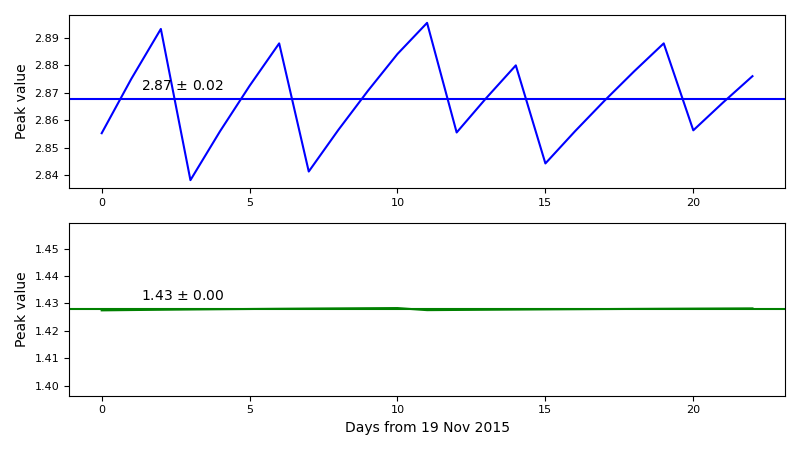
\includegraphics[scale=0.40]{k2/images/period_track.png} \\
\vspace{-.5cm}
\end{center}   
\caption{This shows the variations in the result from the first two peaks
(represented as blue and green) in the periodogram shown over the whole of the
data for the last 40 days (19 November 2015 onward) by taking a 20-day
``window'' of the data starting at successive days.
The scale is kept at the same value for both plots
for comparison.}\protect\label{fig:win20day}
\end{figure}

\begin{figure}[!htbp]
\begin{center}
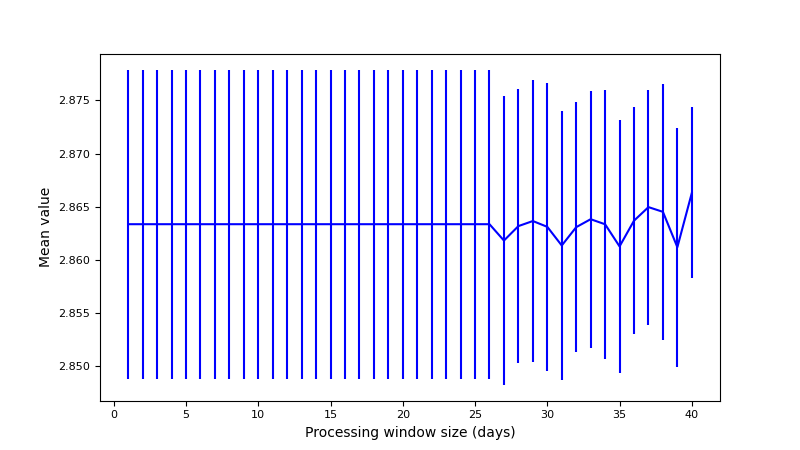
\includegraphics[scale=0.40]{k2/images/k2winsizes.png} \\
\vspace{-.5cm}
\end{center}
\caption{This shows the mean value of the
periodogram main peak (solid line) and the
standard deviations (dotted line, scale on RH
axis), for successive window sizes with the
windows run over the whole data from 19 November
2015.}\protect\label{fig:k2winsizes}
\end{figure}

It would appear that consistent results showing a rotation period of 2.87 $\pm$
0.01 days are obtainable from {\ktwo} and also a ``window'' of up to 20 days is
suitable without errors being introduced due to changes to the surface features.
For any set of data, there will have to be a compromise between the frequency
of observations in a set and minimising the number of days over which the sample is taken.
{\ktwo} has approximately 50 observations recorded each day which is more than enough
to obtain a result over just one day, given the excellent SNR.

\subsection{Studies of data from {\asas}}
\protect\label{section:asas}

{\asas} data is available over approximately a decade, although the observations
are taken less frequently than with \ktwo. A plot of the data is shown in Fig.
\ref{fig:asasall}. Again, flaring data obscures several of the observations, but
it was possible to find a number of periods in the data during which little or no flaring took place. In Fig. \ref{fig:asaslcurve} is
shown one such period and the light curve. A periodogram was produced from this,
showing a peak at 2.87 days as shown in Fig. \ref{fig:asaspgram}. Similar
results were obtained from the other periods which did not appear to be affected
by flaring.

\begin{figure}[!htbp]
\begin{center}
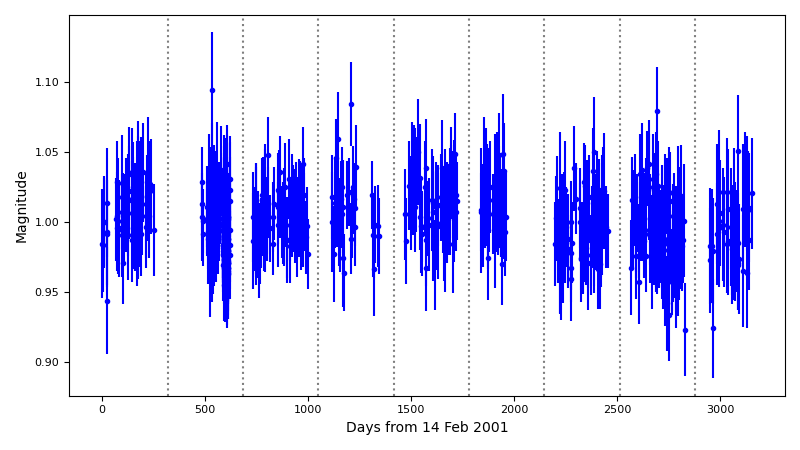
\includegraphics[scale=0.40]{asas/images/asasall.png} \\
\vspace{-.5cm}
\end{center}   
\caption{Data for {\ross} taken from the {\asas} archive selecting only Class A
and B data, converting magnitude and errors to flux values and ignoring data
outside 3 standard deviations from the mean.
The dotted vertical lines show the year divisions. The recommended aperture (2) was used.}\protect\label{fig:asasall}
\end{figure}

\begin{figure}[!htbp]
\begin{center}
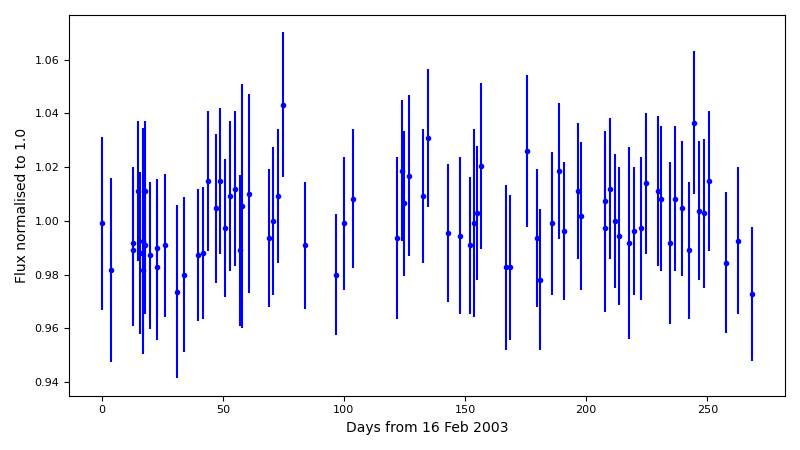
\includegraphics[scale=0.40]{asas/images/asaslcurve.png} \\
\vspace{-.5cm}
\end{center}   
\caption{Subset of Fig. \ref{fig:asasall}, showing {\asas} data for {\ross}
taken from the archive for nearly a year from February 2003, converting
magnitude and errors to flux values and selecting only Class A and B data and
ignoring data outside 3 standard deviations.
This display shows the reported error bar for each observation, the reported magnitude
value being shown as a single point. The
recommended aperture (2) was used.}\protect\label{fig:asaslcurve}
\end{figure}

\begin{figure}[!htbp]
\begin{center}
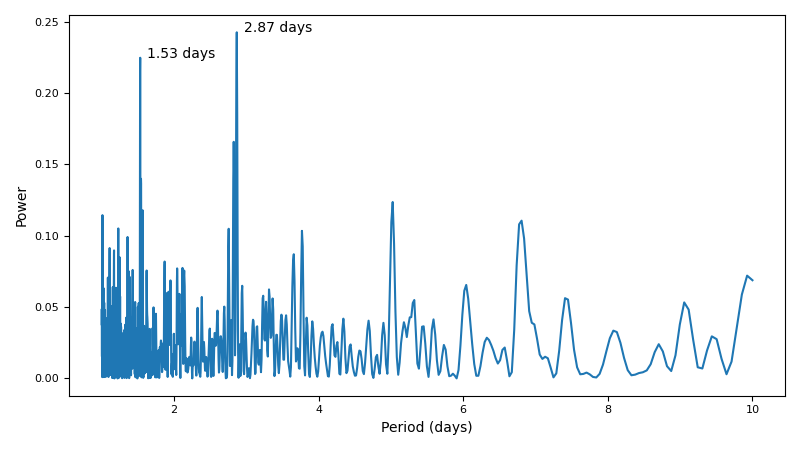
\includegraphics[scale=0.40]{asas/images/asaspgram.png} \\
\vspace{-.5cm}
\end{center}   
\caption{Periodogram taken from the data displayed in Fig.
\ref{fig:asaslcurve}. Again, periods less than 1
day are not considered as the window function (not shown here) reveal numerous
peaks below one day, similar to those shown in Section
\ref{section:k2data}}\protect\label{fig:asaspgram}
\end{figure}

This would again confirm a rotation period of 2.87 days as suggested from the K2
results above in Section \ref{section:k2data}.


\subsection{Studies of data from {\MEarth}}
\protect\label{section:mearth}

A data file of observations from {\MEarth} for {\ross} was obtained, showing
observations taken between 15 April 2015 and 16 November 2015. This are
displayed in Fig. \ref{fig:mearthobs}. A periodogram was obtained over the whole
of the data, as displayed in Fig. \ref{fig:mearthallpgram}.

\begin{figure}[!htbp]
\begin{center}
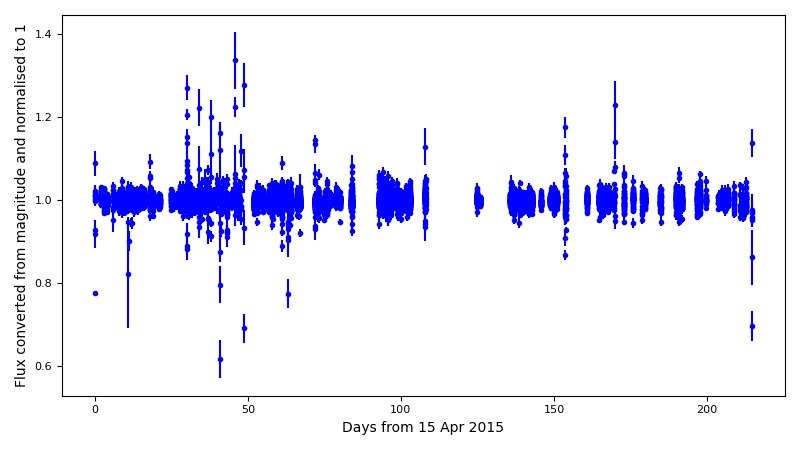
\includegraphics[scale=0.40]{mearth/images/mearthlcurve.png} \\
\vspace{-.5cm}
\end{center}   
\caption{This shows the available observations from
{\MEarth} showing the flux, converted from the reported magnitudes and
normalised to 1, between 15 April and 16 November 2015.}\protect\label{fig:mearthobs}
\end{figure}

\begin{figure}[!htbp]
\begin{center}
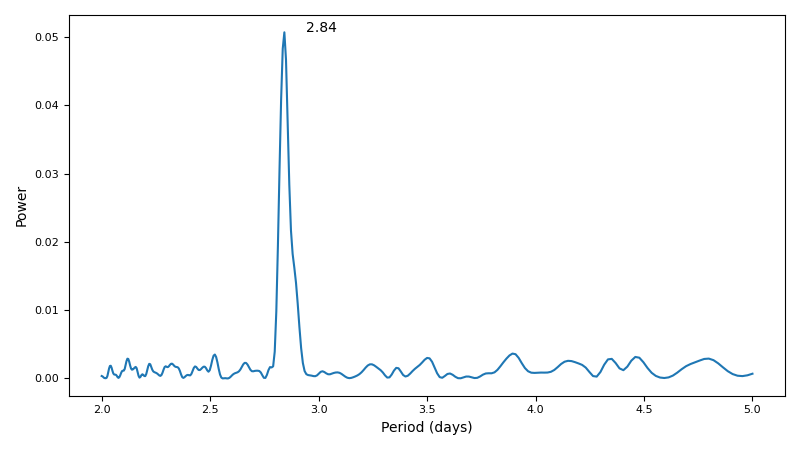
\includegraphics[scale=0.40]{mearth/images/mearthallpgram.png} \\
\vspace{-.5cm}
\end{center}   
\caption{This is a periodogram obtained from
the data in Fig. \ref{fig:mearthobs} for \MEarth. Pruning
of the data of outliers, such as points
exceeding those deviating by more than 2
standard deviations in the data, had
negligible effect on the results.}\protect\label{fig:mearthallpgram}
\end{figure}

The period result of 2.85 days is close to that of 2.843 days obtained from
{\MEarth} by \citet{newton18}. However, the analysis of the {\ktwo} data above
would suggest the the period of approximately 7 months is much too large for an
accurate periodogram; the surface features will have evolved during that period.
There is a problem however in that the number of observations per day is
considerably less than for \ktwo, on some days only of the order of 10
observations were made, less if any are excluded as outliers. In Fig.
\ref{fig:mearthwinsizes} is shown the result of the exercise of trying various
window sizes on the data. It is to be noted that the window function, shown in
Fig. \ref{fig:mearthwinfunc} shows a peak close to this value and possibly
interferes with it.

\begin{figure}[!htbp]
\begin{center}
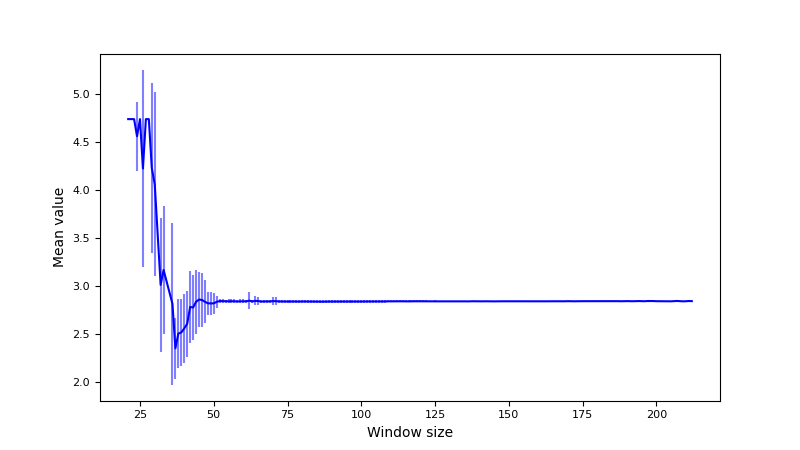
\includegraphics[scale=0.40]{mearth/images/mearthwinsizes.png} \\
\vspace{-.5cm}
\end{center}
\caption{This shows, for the {\MEarth} data for \ross, the development of mean
value of the periodogram main peak (solid line) as the the number of days in
the processing main window is increased. The error bars show the standard
deviations of the mean peak. Points over 2 standard deviations in the data were
omitted from consideration.}\protect\label{fig:mearthwinsizes}
\end{figure}

\begin{figure}[!htbp]
\begin{center}
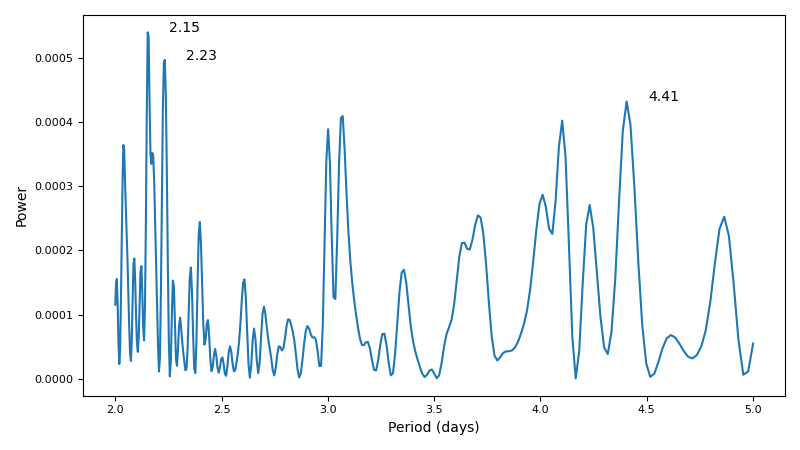
\includegraphics[scale=0.40]{mearth/images/mearthwinf.png} \\
\vspace{-.5cm}
\end{center}
\caption{This shows the window function for
the time series given by the {\MEarth} data
for {\ross} shown in Fig. \ref{fig:mearthobs}
for which the periodogram is shown in Fig.
\ref{fig:mearthallpgram}.}\protect\label{fig:mearthwinfunc}
\end{figure}


\subsection{Studies of data from {\rem}}
\protect\label{section:rem}

In this section is analysed observational data from the
REM (Rapid Eye Mount) telescope and camera equipment in La Silla, Chile, as
operated by the Red Dots Project. The observatory at La Silla was initially set up in 2003
\citep{antonelli05} consisting of the the REMIR near-infrared camera and the
visible light camera, ROSS. Light from the 60cm telescope is split at 1 $\mu$m into two beams
by a dichroic element. The light with wavelength greater than this passes to the
REMIR near-infrared camera and the smaller wavelengths to the ROSS camera.
The performance of the ROSS camera was not satisfactory and in 2015 it
was replaced by the ROSS2 camera system, described in outline at
\citet{reminaf7} and in more detail in \citet{molinari14}.

The work for this paper has focused on the ROSS2 visible light data. The same
patch of sky is viewed via 4 filters on this part of the telescope with exactly
the same exposure, in addition to 3 filters, combined with various dither
patterns by the REMIR telescope.

The REM telescope has been set up to take a series of automatic
observations of patches of sky on a nearly nightly basis. The main concern of
the Red Dots Project is of 3 {\rdwarf} stars, including {\prox} and {\bstar} as
well as \ross, but the REM observatory is concurrently used for other projects,
for example \citet{giannini18}.

The first observations of {\rdwarf} stars took place in mid-2017. All
observations ceased on March 2020 due to the Coronavirus pandemic but were
restarted in October 2020 and have continued up until April 2022. Between 6
August 2017 and 23 March 2022, 48,925 images including {\ross} were taken at
once, with a variety of filters. \texttt{g'}, \texttt{r'}, \texttt{i'} and
\texttt{z'}, hereinafter referred to as \texttt{g}, \texttt{r}, \texttt{i} and
\texttt{z} respectively.

\subsubsection{{\rem} observations of \ross}
\protect\label{section:remross}

Of the REM observations of \ross, 23,236 were taken using visible light filters
5,809 were taken using the \texttt{r} filter and after excluding 412 blank,
excessively noisy or otherwise unusable images, 5,297 were used, taken between 6
August 2017 and 23 March 2022.

Along with the images, a series of bias and flat files were collected daily and
these were used to create master bias and flat files.\footnote{Master monthly
daily flat and bias files were also created by the Red Dots Project, but these
were rejected for a variety of reasons, the most important being that the bias
files, after subtraction, rendered the pixel values negative in places both in
the image files and also in the daily flat files.}

The method of calibration used was to take the mean flux for each reference
star and then for each image and using each reference star within the image
construct a linear regression line. There are typically over 100 reference
stars available in each image, however the subset of reference stars out of the
set of over 600 possible ones for {\ross} is different for each frame as the
orientation of telescope and the position of {\ross} within the frame varies, or
objects are obliterated by cosmics and other issues.

The linear regression technique proved to have a very high correlation of
95\% or more in most cases. It was then possible to map the flux from {\ross}
back to a deviation from the mean and factors such as airmass, moon phase and so
forth consistently eliminated.

After calibration, the flux was calculated for the various observations from each
of the usable frames as shown in Fig \ref{fig:rossallcurve}.

\begin{figure}[!htbp]
\begin{center}
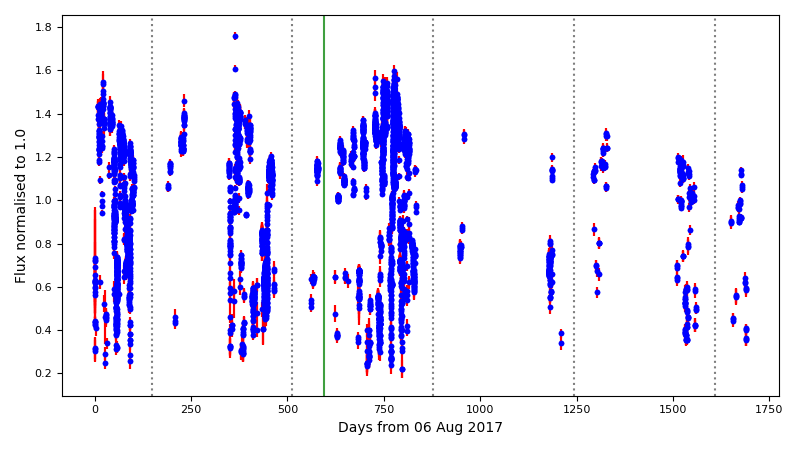
\includegraphics[scale=0.40]{REM/images/remrossallcurve.png} \\
\vspace{-.5cm}
\end{center}   
\caption{This shows the total flux after calibration from {\ross}
found in all acceptable images in {\rem}
observations, normalised so that the mean is 1.0. There was a change in
configuration in late March 2019, indicated by the sold vertical green line, but
this occurred 595 days from the start and thus does
not account for any of the shape of the plot
shown. The dotted vertical lines indicate the
start of the years 2018 through to 2022.}\protect\label{fig:rossallcurve}
\end{figure}

It proved hard to construct a clear periodogram from this data due to the
significant intervals between observations. Also only 4 or 5 observations are done in one
night, sometimes days apart, and this is far too small for any meaningful
results to be obtained. The observations are typically taken nightly at
the same time each night and this introduces a cycle close to the
rotation period. Attempts to produce periodograms from all the data yielded
numerous peaks, very densely packed but samples of observations taken much
closer together were more acceptable. In Fig.
\ref{fig:rossallpgram} is shown the portion between 2 and 5 days for the observations taken during 2022.

\begin{figure}[!htbp]
\begin{center}
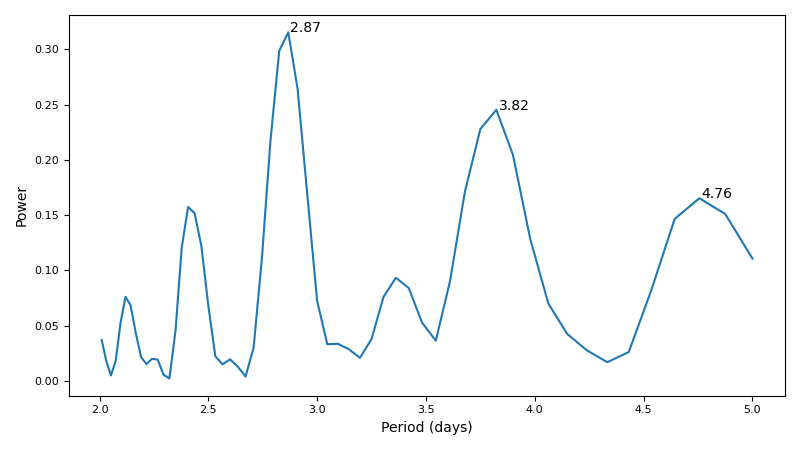
\includegraphics[scale=0.40]{REM/images/rem2022pgram.png} \\
\vspace{-.5cm}
\end{center}   
\caption{This shows part of the periodogram derived from the the data shown in
Fig. \ref{fig:rossallcurve} pertaining to 2022 (up
to 23 March), restricting the display to 2 to 5 days.}\protect\label{fig:rossallpgram}
\end{figure}

\IfThesis{
\subsubsection{Improving the {\rem} observation calibration}
\protect\label{section:remrosscalib}

The above flux from {\ross} was just on the flux alone, but did not take into
account other stars and factors such as air mass, weather and other influences
on the flux. By identifying the other stars in the object, discarding variable
and irregularly-shaped objects, such as binary or objects closer together than
the telescope resolution (approximately 0.6 arc second per pixel) could separate,
the remaining objects could be ordered, in descending brightness and also by
frequency of occurrence in the images, (as some of the possible reference stars
were outside the edges of the image for some frames).

A periodogram was produced from this parallel to that in Fig.
\ref{fig:rossallpgram} in Fig. \ref{fig:rosscombpgram}. The result is seen to
have considerably less peaks than in the former figure, but the main peak is
consistently displaced to 2.91 days from 2.87 days. This was repeated for
different periods and different selections of reference stars with almost
identical results.


\begin{figure}[!htbp]
\begin{center}
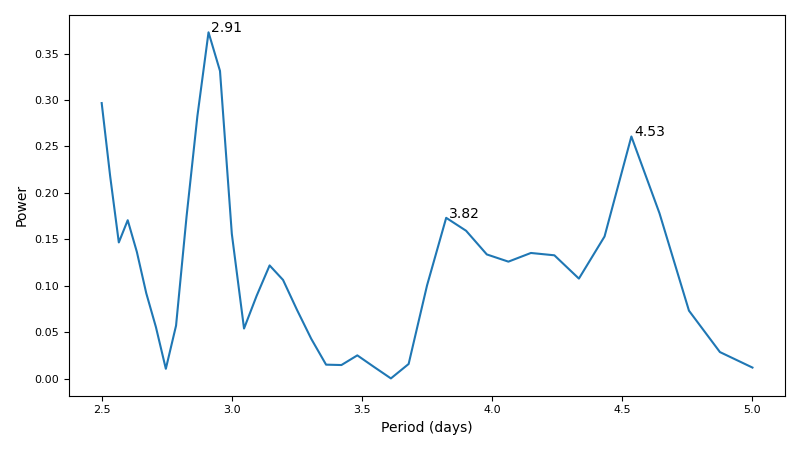
\includegraphics[scale=0.40]{REM/images/remcomb2022pgram.png} \\
\vspace{-.5cm}
\end{center}   
\caption{This shows part of the periodogram derived by starting from the
same data as in Fig. \ref{fig:rossallcurve} pertaining
to 2022 (up to 23 March), but calculating the ratio of the flux to
the sum of that from the 4 brightest stars common to all of the
images again restricting the display to 2.5 to 5 days.}\protect\label{fig:rosscombpgram}
\end{figure}

There is a suggestion of a longer period in Fig. \ref{fig:rossallcurve} which is
not observed in light curve plots for other objects, and Fig.
\ref{fig:rosslongperiod} shows a periodogram for periods between 500 and 2,000
days.

\begin{figure}[!htbp]
\begin{center}
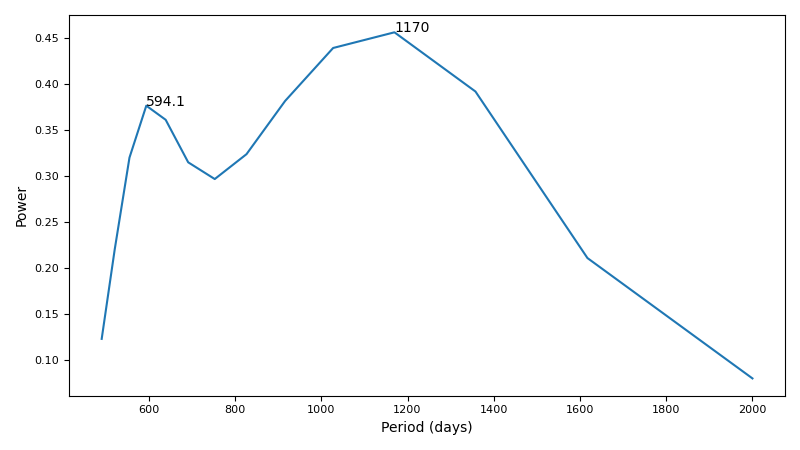
\includegraphics[scale=0.40]{REM/images/rosslongperiod.png} \\
\vspace{-.5cm}
\end{center}   
\caption{This shows the periodogram taken
over the whole of the data (as shown in Fig.
\ref{fig:rossallcurve}) showing peaks in the
range of 500 to 2,000 days.}\protect\label{fig:rosslongperiod}
\end{figure}

There are insufficiently long periods recorded in the {\rem} observations or
other data for this periodicity to be explored further.}

\subsubsection{Specific conclusions as to the {\rem} images}
\protect\label{section:remconclusions}

\IfThesis{
An important step in improvement of the {\rem} image processing would be to
improve the handling of reference stars by a linear regression of the expected flux derived
from the published or empirically-computed magnitudes to the observed flux for
each of the reference stars involved.} 

There is further work to be done in improving and tuning the aperture selection
for each of the reference stars and removing those found to be excessively
variable, notwithstanding any lack of indication of variability from the
catalogues. It is not anticipated that this will have a significant effect on
the periodogram results.

It is also necessary to improve the calibration files by better eliminating
defective pixels from the images and refining the uncertainty on an individual
pixel basis. This is not anticipated to make a large difference either.

However, it does not seem to be possible to improve the performance of the
{\rem} image processing significantly, to be confident of calculating rather
than merely confirming the figure derived from other methods.
It may well be that refinements to the calculations, especially with the
reference star classification of which over 600 were considered for \ross, may
yield better results, It should also be noted that {\ross} is on average nearly
70 times brighter in the images than the other objects. The uncertainty for the
{\ross} observations is approximately 0.27\% in the images, but that for the
other objects averages out at approximately 13\% due to the lack of contrast
between the objects and the sky level.

There might be scope for improvements by increasing the exposure times for the
images taken by the {\rem} telescope. This could be conveniently doubled without
risking saturation on the most useful filter images.

\section{Discussion and conclusions}
\protect\label{section:discussion}

A survey of the data used in other papers confirms the rotation period of $2.87
\pm 0.01$ days derived in most of the papers reviewed and this period is
also confirmed by the processing of the {\rem} data.

The lack of contrast in the {\rem} images is unfortunate, but could be improved
by increasing the exposure time, which would improve the SNR considerably,
especially for the fainter reference stars.

Nevertheless, it is clear that it is possible to recover the same period,
believed to be the rotation period, from \ross.

Further developments in the processing of {\rem} data will include consideration
of the other target \rdwarf s, {\prox} and {\bstar} in addition to the other
filters and the REMIR data. The optical filters \texttt{g}. \texttt{i} and \texttt{z} are likely to be
less promising than \texttt{r}, however as \texttt{g} is on a much noisier
portion of the CCD and the other too filters do not show nearly as many
reference stars as the \texttt{g} and \texttt{r} filters.

\section{Acknowledgements}

All the figures were produced \refrevision{via Python programs developed by the authors using the {\matplot} libary}, which is
associated with the {\scipy} library \citep{jones01}.

\Notnow{{\FirstP} are grateful to the anonymous referee for his or her kind
assistance in recommending significant improvements to prepare this paper for
publication.}

Hugh R.A. Jones and John R. Barnes were supported by the Science and Technology Facilities Council grants ST/M001008/1
and ST/L000776/1 and Hugh R.A. Jones also by Leverhulme Trust grant, RPG-
2014-281.

\textit{Need something about Ben}


\bibliographystyle{aa}
\bibpunct{(}{)}{;}{a}{}{,} % to follow the A&A style
%\bibpunct{(}{)}{;}{s}{,}{,}
\bibliography{bibrefs}

\protect\label{lastpage}
\end{document}
